\documentclass[twoside]{article}
\usepackage{amsgen,amsmath,amstext,amsbsy,amsopn,amssymb,}
\usepackage{graphicx}
\usepackage{epsfig}

\setlength{\oddsidemargin}{0.1 in} \setlength{\evensidemargin}{-0.1
in} \setlength{\topmargin}{-0.6 in} \setlength{\textwidth}{6.5 in}
\setlength{\textheight}{10 in} \setlength{\headsep}{0.1 in}
\setlength{\parindent}{0 in} \setlength{\parskip}{0.1 in}

\newcommand{\homework}[2]{
   \pagestyle{myheadings}
   \thispagestyle{plain}
   \newpage
   \setcounter{page}{1}
   \noindent
   \begin{center}
   \framebox{
      \vbox{\vspace{2mm}
       \hbox to 6.28in { {\bf Math 4720:~Statistical Methods \hfill} }
       \vspace{6mm}
       \hbox to 6.28in { {\Large \hfill #1 (#2)  \hfill} }
       \vspace{6mm}
      \vspace{2mm}}
   }
   \end{center}
   \markboth{#1}{#1}
   \vspace*{4mm}
}

\newcommand{\bbF}{\mathbb{F}}
\newcommand{\bbX}{\mathbb{X}}
\newcommand{\bI}{\mathbf{I}}
\newcommand{\bX}{\mathbf{X}}
\newcommand{\bY}{\mathbf{Y}}
\newcommand{\bepsilon}{\boldsymbol{\epsilon}}
\newcommand{\balpha}{\boldsymbol{\alpha}}
\newcommand{\bbeta}{\boldsymbol{\beta}}
\newcommand{\0}{\mathbf{0}}

\begin{document}

\homework{$2^{nd}$ Week Summary}{01/24/25}
\begin{itemize}
\item Relationship between two variables :
\item Explanatory and response variables
\subitem Categorical vs. Quantitative : side-by-side box-plot
\subitem Quantitative vs. Quantitative : correlation $r=\dfrac{1}{n-1}\sum_{i=1}^n\Biggl(\dfrac{x_i-\bar{x}}{s_x}\Biggr)\Biggl(\dfrac{y_i-\bar{y}}{s_y}\Biggr)$
\item Properties of the Correlation r:
\subitem Takes values between $-1$ and $1$
\subitem $r = 1$ or $r = -1$ implies that the points lie on a straight line
\subitem $r = 0$ implies that there is no \textbf{linear} association
\subitem $r < 0$ implies that there is a negative \textbf{linear} association \& $r > 0$ implies positive \textbf{linear} association
\subitem If the x and y variables are switched, the correlation will stay the same
\subitem r does not change when we change the units of measurement of $x, y$, or both.
\subitem r is strongly affected by a few outliers.
\item \textbf{Chapter 3: Probability}
\item The \textbf{probability} of any event A of a random phenomenon is the proportion of times the event would occur in a very long series of repetitions.
\item The \textbf{sample space $S$} of a random phenomenon is the set of all possible outcomes.
\item An \textbf{event} is a subset of the sample space.
\item Probability Rules
\subitem The probability $P(A)$ of any event $A$ satisfies $0 < P(A) < 1$.
\subitem If $S$ is the sample space, then $P(S) = 1$.
\subitem Two events $A$ and $B$ are \textbf{disjoint} if they have no outcomes in common and so can never occur together. If $A$ and $B$ are disjoint, $P(A \ \textrm{or} \ B) = P(A \bigcup B) = P(A) + P(B)$
\subitem For any event $A$, $P(A$ does not occur$) = P(\overline{A}) = 1 - P(A)$.
\item Addition rule in general : $P(A \ \textrm{or} \ B) = P(A \bigcup B) = P(A) + P(B) - P( A \bigcap B )$

\begin{figure}[h]
\begin{center}
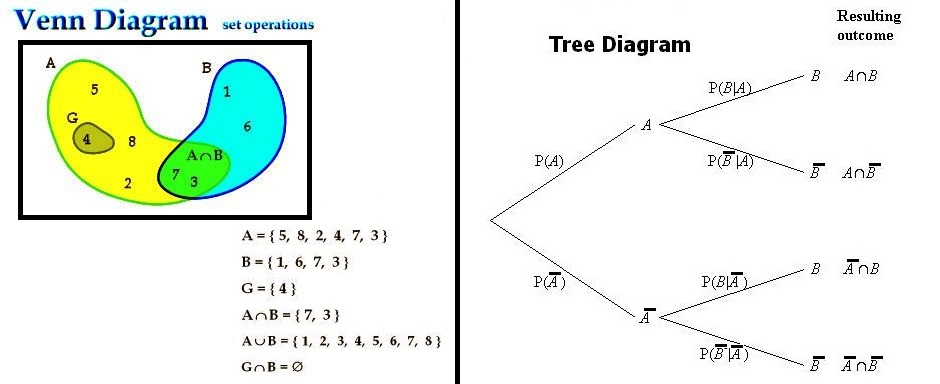
\includegraphics[angle=0,width=5.5in] {venn_tree.jpg}
\end{center}
\end{figure}
\end{itemize}

\end{document}
